\documentclass[tikz,border=10pt]{standalone}
\usepackage{tikz}
\usetikzlibrary{positioning,arrows.meta,shapes.geometric}

\begin{document}
% System Architecture Diagram - Figure 4.1
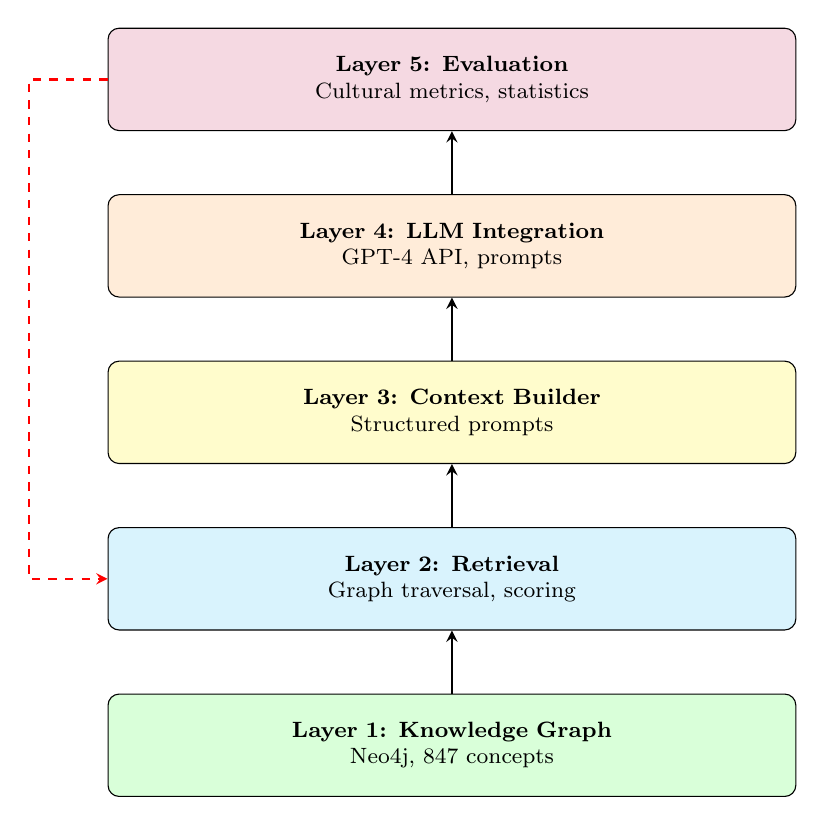
\begin{tikzpicture}[
    node distance=0.8cm,
    layer/.style={rectangle, draw, fill=blue!10, text width=8.5cm, minimum height=1.3cm, align=center, rounded corners, font=\footnotesize},
    arrow/.style={->, >=stealth, thick},
]

% Layers
\node[layer, fill=purple!15] (eval) at (0,0) {\textbf{Layer 5: Evaluation} \\ Cultural metrics, statistics};
\node[layer, fill=orange!15, below=of eval] (llm) {\textbf{Layer 4: LLM Integration} \\ GPT-4 API, prompts};
\node[layer, fill=yellow!20, below=of llm] (context) {\textbf{Layer 3: Context Builder} \\ Structured prompts};
\node[layer, fill=cyan!15, below=of context] (retrieval) {\textbf{Layer 2: Retrieval} \\ Graph traversal, scoring};
\node[layer, fill=green!15, below=of retrieval] (kg) {\textbf{Layer 1: Knowledge Graph} \\ Neo4j, 847 concepts};

% Arrows
\draw[arrow] (kg) -- (retrieval);
\draw[arrow] (retrieval) -- (context);
\draw[arrow] (context) -- (llm);
\draw[arrow] (llm) -- (eval);
\draw[arrow, dashed, red] (eval.west) -- ++(-1,0) |- (retrieval.west);

\end{tikzpicture}
\end{document}
